\chapter{Experiment and Result}
brief of experiment and result.
\section{Experiment}
Please tell how the experiment conducted from method.

\section{Result}
Please provide the result of experiment

\section{Ahmad Syafrizal Huda/1164062}
\subsection{Teori}
\begin{enumerate}
\item Klasifikasi teks adalah proses pemberian kategori ke dalam teks/dokumen sesuai dengan tipikal dalam supervised machine
\par learning (ML) yang bisa berupa buku perpustakaan, halaman web, artikel media, galeri, dan lain sebagainya. Tujuannya 
\par untuk memberikan label pada setiap teks/dokumen.
\par Contoh ilustrasi gambar dapat dilihat pada gambar \ref{c4_1}
\begin{figure}[ht]
	\centerline{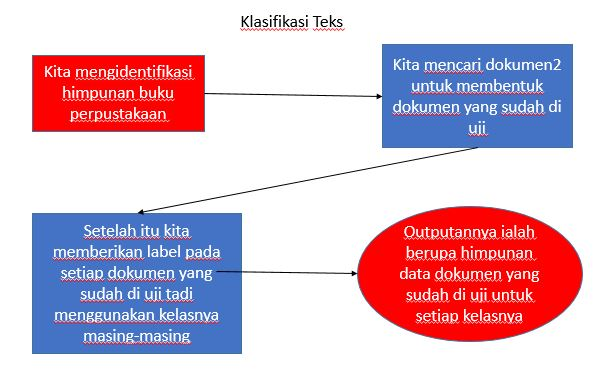
\includegraphics[width=1\textwidth]{figures/huda/chapter4/1.JPG}}
	\caption{Klasifikasi Teks}
	\label{c4_1}
\end{figure}
\item Mengapa klasifikasi bunga tidak dapat menggunakan machine learning? itu dikarenakan memiliki masalah masukan(input) 
\par yang sama tetapi keluarannya (output) yang berbeda, biasanya output yang berbeda ini disebut dengan istilah 'noise'.
\par Noise berarti output yang disimpan bukan seperti seharusnya ( keluaran yang tidak diinginkan ). 
\par Contoh ilustrasi gambar dapat dilihat pada gambar \ref{c4_2}
\begin{figure}[ht]
	\centerline{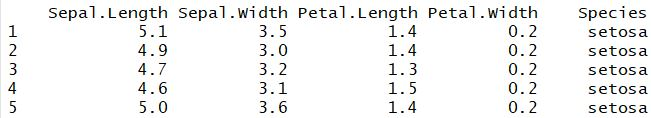
\includegraphics[width=1\textwidth]{figures/huda/chapter4/2.JPG}}
	\caption{Klasifikasi Bunga}
	\label{c4_2}
\end{figure}
\item Teknik pembelajaran mesin pada teks biasanya menggunakan teknik bag-of-words pada klasifikasi berbasis text dan kata 
\par untuk mengklasifikasikan komentar yang ada diinternet sebagai spam atau bukan. Misalkan pada kolom komentar di youtube
\par dapat di cek seberapa sering suatu kata muncul dalam kalimat. Setiap kata dapat dijadikan baris dan kolomn yang 
\par merupakan kategori kata tersebut, apakah masuk kedalam spam atau tidak. dan contoh lainnya yaitu pada Caption. dimana
\par akan muncul subtitle secara otomatis dari youtube menggunakan sensor suara yang disesuaikan dengan kata yang telah 
\par ditentukan. 
\par Contoh ilustrasi gambar dapat dilihat pada gambar \ref{c4_3}
\begin{figure}[ht]
	\centerline{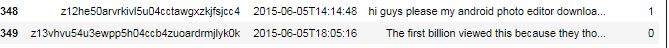
\includegraphics[width=1\textwidth]{figures/huda/chapter4/3.JPG}}
	\caption{Comment Youtube}
	\label{c4_3}
\end{figure}
\item Vektorisasi data merupakan pembagian dan pemecahan data yang kemudian nantinya data tersebut akan menjadi beberapa data
\par Contoh misalkan dari sebuah paragraph nantinya kan di pecah menjadi beberapa kalimat dari kalimat tersebut dibagi lagi
\par menjadi beberapa kata.
\item Bag-of-words adalah cara untuk merepresentasikan data teks saat memodelkan teks yang menggambarkan kemunculan 
\par kata-kata dalam dokumen dengan algoritma pembelajaran mesin.
\par Contoh ilustrasi gambar dapat dilihat pada gambar \ref{c4_4}
\begin{figure}[ht]
	\centerline{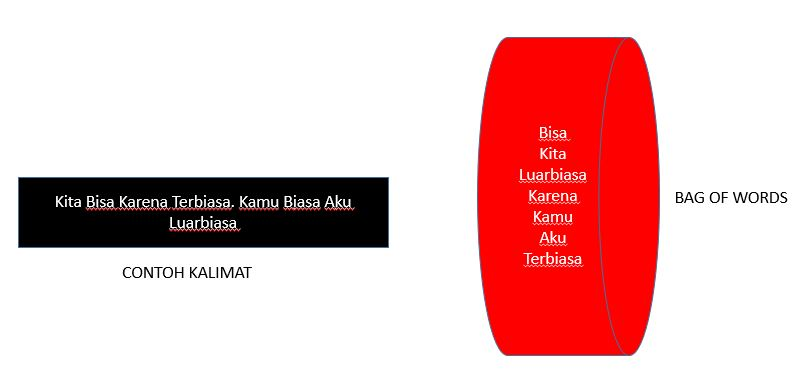
\includegraphics[width=1\textwidth]{figures/huda/chapter4/4.JPG}}
	\caption{Bag Of Words}
	\label{c4_4}
\end{figure}
\item TF-IDF  memberi kita frekuensi kata dalam setiap dokumen atau mengganti data jadi number. Ini adalah rasio berapa 
\par kali kata itu muncul dalam dokumen dibandingkan dengan jumlah total kata dalam dokumen itu. Itu meningkat seiring 
\par jumlah kemunculan kata itu di dalam dokumen meningkat. Setiap dokumen memiliki tf sendiri.
\par Contoh ilustrasi gambar dapat dilihat pada gambar \ref{c4_5}
\begin{figure}[ht]
	\centerline{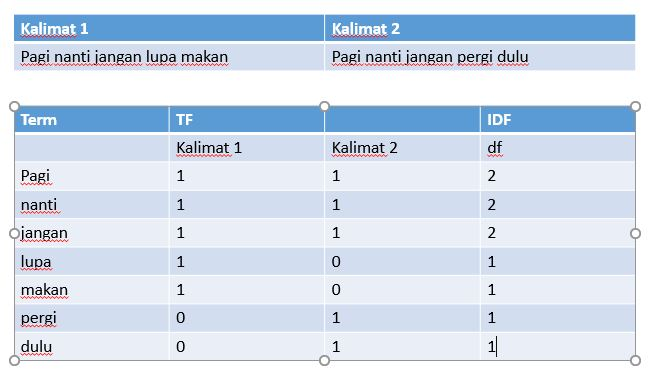
\includegraphics[width=1\textwidth]{figures/huda/chapter4/5.JPG}}
	\caption{TF-IDF}
	\label{c4_5}
\end{figure}
\end{enumerate}